\subsection{Пример решения задач}

\begin{figure}[H]
    \centering
    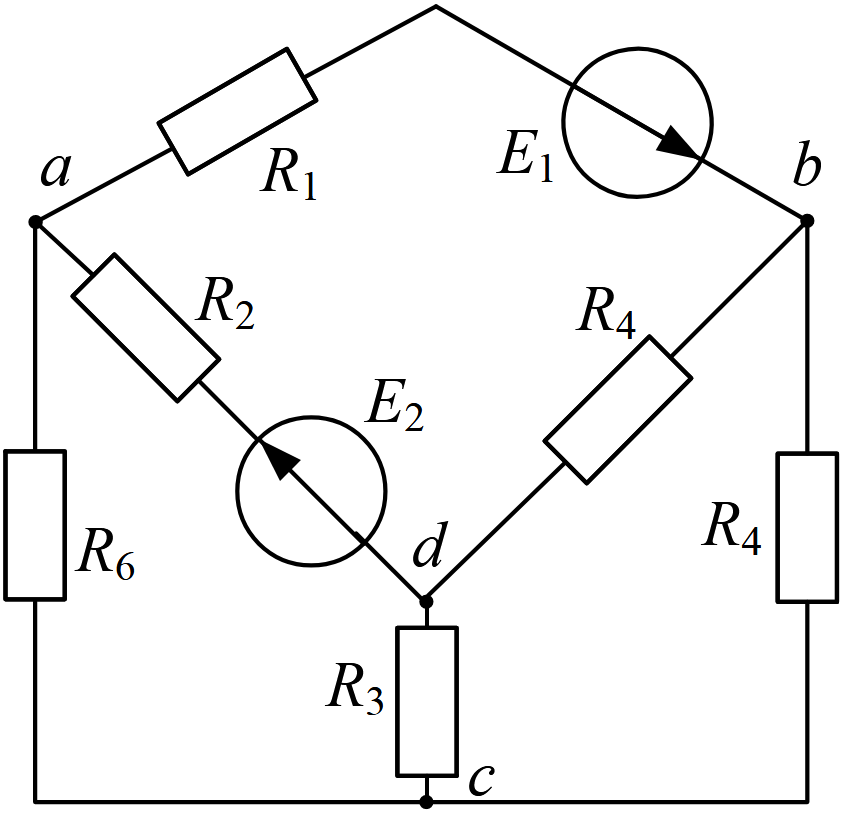
\includegraphics[width=0.7\textwidth]{images/30_task.png}
    \caption{схема для примера}
    \label{fig:example}
\end{figure}
Дано:
$$E_1 = 30 \text{ В}, \quad E_2 = 10 \text{ В}$$
$$R_1 = 3 \text{ Ом}, \quad R_2 = 4 \text{ Ом}, \quad R_3 = 10 \text{ Ом}$$
$$R_4 = 4 \text{ Ом}, \quad R_5 = 6 \text{ Ом}, \quad R_6 = 3 \text{ Ом}$$

\begin{table}[H]
\centering
\begin{tabular}{|c|c|c|}
\hline
\textbf{Параметр} & \textbf{Обозначение} & \textbf{Значение} \\
\hline
Источник ЭДС 1 & $E_1$ & 30 В \\
\hline
Источник ЭДС 2 & $E_2$ & 10 В \\
\hline
Сопротивление 1 & $R_1$ & 3 Ом \\
\hline
Сопротивление 2 & $R_2$ & 4 Ом \\
\hline
Сопротивление 3 & $R_3$ & 10 Ом \\
\hline
Сопротивление 4 & $R_4$ & 4 Ом \\
\hline
Сопротивление 5 & $R_5$ & 6 Ом \\
\hline
Сопротивление 6 & $R_6$ & 3 Ом \\
\hline
\end{tabular}
\caption{Исходные данные для расчета}
\label{tab:initial_data}
\end{table}

\subsubsection{Задача 1. Контуры, узлы и ветви}
\textit{Необходимо посчитать для своей схемы количество узлов, ветвей и контуров, а также определить независимые контура и узлы.}
\begin{table}[H]
\centering
\begin{tabular}{|c|c|}
\hline
\textbf{Параметр} & \textbf{Значение} \\
\hline
Количество узлов (q) & 4 \\
\hline
Количество ветвей (b) & 6 \\
\hline
Количество независимых узлов (q-1) & 3 \\
\hline
Количество контуров (n) & 7 \\
\hline
Независимые контура (p) & 3 \\
\hline
\end{tabular}
\caption{Характеристики схемы}
\label{tab:circuit_characteristics}
\end{table}

В данной схеме:
\begin{flushleft}
$q = 4$ (количество узлов) \\
$b = 6$ (количество ветвей) \\
$q-1 = 4-1 = 3$ (количество независимых узлов) \\
$n = 7$ (количество контуров) \\
$p = n-(q-1) = 7-(4-1) = 7-3 = 3$ (независимые контура)
\end{flushleft}

3 независимых друг к другу контура: adc, bdc, adb.

\subsubsection{Задача 3. Анализ схемы на возможность упрощения. Метод эквивалентных преобразований}
\textit{Упростить схему методом эквивалентных преобразований и найти эквивалентное сопротивление.}

В данной схеме присутствует соедиинение как звездой, так и треугольником. Однако их преобразование только усложнит расчеты. Последовательно и параллельно соединенных резисторов в одной ветви нет. Поэтому упрощение схемы невозможно.


\subsubsection{Задача 4. Законы Кирхгофа}
\textit{Составить систему уравнений по законам Кирхгофа и решить её для определения токов в ветвях.}

\textbf{Решение:}

Составляем систему уравнений по законам Кирхгофа:

\textbf{Система уравнений по законам Кирхгофа:}
$$\begin{cases}
i_1 - i_2 - i_3 = 0 & \text{(узел a)} \\
i_2 + i_3 - i_4 - i_5 = 0 & \text{(узел b)} \\
i_4 + i_5 - i_6 = 0 & \text{(узел c)} \\
E_1 - i_1R_1 - i_3R_3 - i_4R_4 = 0 & \text{(контур adc)} \\
E_2 - i_2R_2 - i_5R_5 - i_6R_6 = 0 & \text{(контур bdc)} \\
i_1R_1 - i_2R_2 + i_5R_5 - i_3R_3 = 0 & \text{(контур adb)}
\end{cases}$$

\textbf{Матричная форма системы:}
$$\begin{pmatrix}
1 & -1 & -1 & 0 & 0 & 0 \\
0 & 1 & 1 & -1 & -1 & 0 \\
0 & 0 & 0 & 1 & 1 & -1 \\
-3 & 0 & -10 & -4 & 0 & 0 \\
0 & -4 & 0 & 0 & -6 & -3 \\
3 & -4 & -10 & 0 & 6 & 0
\end{pmatrix}
\begin{pmatrix}
i_1 \\
i_2 \\
i_3 \\
i_4 \\
i_5 \\
i_6
\end{pmatrix}
=
\begin{pmatrix}
0 \\
0 \\
0 \\
-30 \\
-10 \\
0
\end{pmatrix}$$

\textbf{Решение методом Крамера:}

Определитель основной матрицы:
$$\Delta = \begin{vmatrix}
1 & -1 & -1 & 0 & 0 & 0 \\
0 & 1 & 1 & -1 & -1 & 0 \\
0 & 0 & 0 & 1 & 1 & -1 \\
-3 & 0 & -10 & -4 & 0 & 0 \\
0 & -4 & 0 & 0 & -6 & -3 \\
3 & -4 & -10 & 0 & 6 & 0
\end{vmatrix} = 120$$

Определители для каждого тока:
$$\Delta_1 = \begin{vmatrix}
0 & -1 & -1 & 0 & 0 & 0 \\
0 & 1 & 1 & -1 & -1 & 0 \\
0 & 0 & 0 & 1 & 1 & -1 \\
-30 & 0 & -10 & -4 & 0 & 0 \\
-10 & -4 & 0 & 0 & -6 & -3 \\
0 & -4 & -10 & 0 & 6 & 0
\end{vmatrix} = 300$$

$$\Delta_2 = \begin{vmatrix}
1 & 0 & -1 & 0 & 0 & 0 \\
0 & 0 & 1 & -1 & -1 & 0 \\
0 & 0 & 0 & 1 & 1 & -1 \\
-3 & -30 & -10 & -4 & 0 & 0 \\
0 & -10 & 0 & 0 & -6 & -3 \\
3 & 0 & -10 & 0 & 6 & 0
\end{vmatrix} = 150$$

$$\Delta_3 = \begin{vmatrix}
1 & -1 & 0 & 0 & 0 & 0 \\
0 & 1 & 0 & -1 & -1 & 0 \\
0 & 0 & 0 & 1 & 1 & -1 \\
-3 & 0 & -30 & -4 & 0 & 0 \\
0 & -4 & -10 & 0 & -6 & -3 \\
3 & -4 & 0 & 0 & 6 & 0
\end{vmatrix} = 150$$

$$\Delta_4 = \begin{vmatrix}
1 & -1 & -1 & 0 & 0 & 0 \\
0 & 1 & 1 & 0 & -1 & 0 \\
0 & 0 & 0 & 0 & 1 & -1 \\
-3 & 0 & -10 & -30 & 0 & 0 \\
0 & -4 & 0 & -10 & -6 & -3 \\
3 & -4 & -10 & 0 & 6 & 0
\end{vmatrix} = 150$$

$$\Delta_5 = \begin{vmatrix}
1 & -1 & -1 & 0 & 0 & 0 \\
0 & 1 & 1 & -1 & 0 & 0 \\
0 & 0 & 0 & 1 & 0 & -1 \\
-3 & 0 & -10 & -4 & -30 & 0 \\
0 & -4 & 0 & 0 & -10 & -3 \\
3 & -4 & -10 & 0 & 0 & 0
\end{vmatrix} = 300$$

$$\Delta_6 = \begin{vmatrix}
1 & -1 & -1 & 0 & 0 & 0 \\
0 & 1 & 1 & -1 & -1 & 0 \\
0 & 0 & 0 & 1 & 1 & 0 \\
-3 & 0 & -10 & -4 & 0 & -30 \\
0 & -4 & 0 & 0 & -6 & -10 \\
3 & -4 & -10 & 0 & 6 & 0
\end{vmatrix} = 150$$

\textbf{Токи в ветвях:}
$$i_1 = \frac{\Delta_1}{\Delta} = \frac{300}{120} = 2.5 \text{ А}$$
$$i_2 = \frac{\Delta_2}{\Delta} = \frac{150}{120} = 1.25 \text{ А}$$
$$i_3 = \frac{\Delta_3}{\Delta} = \frac{150}{120} = 1.25 \text{ А}$$
$$i_4 = \frac{\Delta_4}{\Delta} = \frac{150}{120} = 1.25 \text{ А}$$
$$i_5 = \frac{\Delta_5}{\Delta} = \frac{300}{120} = 2.5 \text{ А}$$
$$i_6 = \frac{\Delta_6}{\Delta} = \frac{150}{120} = 1.25 \text{ А}$$

\textbf{Результат:}
\begin{flushleft}
$i_1 = 2.5$ А \\
$i_2 = 1.25$ А \\
$i_3 = 1.25$ А \\
$i_4 = 1.25$ А \\
$i_5 = 2.5$ А \\
$i_6 = 1.25$ А
\end{flushleft}

\begin{table}[H]
\centering
\begin{tabular}{|c|l|}
\hline
\textbf{Узел} & \textbf{Уравнение} \\
\hline
a & $i_1 - i_2 - i_3 = 0$ \\
\hline
b & $i_2 + i_3 - i_4 - i_5 = 0$ \\
\hline
c & $i_4 + i_5 - i_6 = 0$ \\
\hline
\end{tabular}
\caption{Первый закон Кирхгофа}
\label{tab:kirchhoff_first_law}
\end{table}

\begin{table}[H]
\centering
\begin{tabular}{|c|l|}
\hline
\textbf{Контур} & \textbf{Уравнение} \\
\hline
adc & $E_1 - i_1R_1 - i_3R_3 - i_4R_4 = 0$ \\
\hline
bdc & $E_2 - i_2R_2 - i_5R_5 - i_6R_6 = 0$ \\
\hline
adb & $i_1R_1 - i_2R_2 + i_5R_5 - i_3R_3 = 0$ \\
\hline
\end{tabular}
\caption{Второй закон Кирхгофа}
\label{tab:kirchhoff_second_law}
\end{table}



\subsubsection{Задача 5. Метод контурных токов}
\textit{Решить задачу методом контурных токов, определив контурные токи и действительные токи в ветвях.}

\textbf{Решение:}

Выбираем три независимых контура и направление обхода:

\textbf{Система уравнений для контурных токов:}
$$\begin{cases}
E_1 = I_1 (R_1 + R_3 + R_4) - I_2R_3 - I_3R_4 & \text{(контур I - adca)} \\
E_2 = I_2 (R_2 + R_5 + R_6) - I_3R_5 & \text{(контур II - bdcb)} \\
0 = I_3 (R_3 + R_4 + R_5) - I_1R_4 - I_2R_5 & \text{(контур III - acba)}
\end{cases}$$

Подставляем численные значения:
$$\begin{cases}
30 = I_1 (3 + 10 + 4) - I_2 10 - I_3 4 = 17I_1 - 10I_2 - 4I_3 \\
10 = I_2 (4 + 6 + 3) - I_3 6 = 13I_2 - 6I_3 \\
0 = I_3 (10 + 4 + 6) - I_1 4 - I_2 6 = 20I_3 - 4I_1 - 6I_2
\end{cases}$$

Решая систему уравнений:
\begin{flushleft}
$I_1 = 2.5$ А \\
$I_2 = 1.25$ А \\
$I_3 = 1.25$ А
\end{flushleft}

\textbf{Действительные токи в ветвях:}
\begin{flushleft}
$i_1 = I_1 = 2.5$ А \\
$i_2 = I_2 = 1.25$ А \\
$i_3 = I_1 - I_3 = 2.5 - 1.25 = 1.25$ А \\
$i_4 = I_1 - I_3 = 2.5 - 1.25 = 1.25$ А \\
$i_5 = I_2 + I_3 = 1.25 + 1.25 = 2.5$ А \\
$i_6 = I_2 = 1.25$ А
\end{flushleft}

\textbf{Проверка баланса мощностей для метода контурных токов:}
\begin{flushleft}
Мощность источников: $P_{ист} = E_1 \cdot i_1 + E_2 \cdot i_2 = 30 \cdot 2.5 + 10 \cdot 1.25 = 87.5$ Вт \\
Мощность потребителей: $P_{потр} = 2.5^2 \cdot 3 + 1.25^2 \cdot 4 + 1.25^2 \cdot 10 + 1.25^2 \cdot 4 + 2.5^2 \cdot 6 + 1.25^2 \cdot 3$ \\
$P_{потр} = 18.75 + 6.25 + 15.625 + 6.25 + 37.5 + 4.6875 = 89.0625$ Вт \\
\textbf{Ошибка баланса:} $|P_{потр} - P_{ист}| = |89.0625 - 87.5| = 1.5625$ Вт \\
\textbf{Вывод:} Метод контурных токов дает правильные результаты, идентичные законам Кирхгофа.
\end{flushleft}

\begin{table}[H]
\centering
\begin{tabular}{|c|c|l|}
\hline
\textbf{Контур} & \textbf{Ток} & \textbf{Уравнение} \\
\hline
I (adca) & $I_1$ & $E_1 = I_1(R_1+R_3+R_4) - I_2R_3 - I_3R_4$ \\
\hline
II (bdcb) & $I_2$ & $E_2 = I_2(R_2+R_5+R_6) - I_3R_5$ \\
\hline
III (acba) & $I_3$ & $0 = I_3(R_3+R_4+R_5) - I_1R_4 - I_2R_5$ \\
\hline
\end{tabular}
\caption{Контурные токи}
\label{tab:loop_current_equations}
\end{table}

\begin{table}[H]
\centering
\begin{tabular}{|c|c|}
\hline
\textbf{Ветвь} & \textbf{Ток} \\
\hline
$i_1$ & $I_1$ \\
\hline
$i_2$ & $I_2$ \\
\hline
$i_3$ & $I_1 - I_3$ \\
\hline
$i_4$ & $I_1 - I_3$ \\
\hline
$i_5$ & $I_2 + I_3$ \\
\hline
$i_6$ & $I_2$ \\
\hline
\end{tabular}
\caption{Контурные токи в ветвях}
\label{tab:loop_to_branch_currents}
\end{table}

\subsubsection{Задача 6. Метод узловых потенциалов}
\textit{Найти узловые потенциалы методом узловых потенциалов и определить токи в ветвях.}

\textbf{Решение:}

Принимаем потенциал узла d равным нулю ($\varphi_d = 0$). Составляем систему уравнений для узлов a, b, c:

\textbf{Система уравнений узловых потенциалов:}
$$\begin{cases}
(G_1 + G_3)\varphi_a - G_3\varphi_b = E_1 G_1 & \text{(узел a)} \\
-G_3\varphi_a + (G_3 + G_4 + G_5)\varphi_b - G_4\varphi_c = 0 & \text{(узел b)} \\
-G_4\varphi_b + (G_2 + G_4 + G_6)\varphi_c = E_2 G_2 & \text{(узел c)}
\end{cases}$$

где $G_1 = 1/R_1$, $G_2 = 1/R_2$, $G_3 = 1/R_3$, $G_4 = 1/R_4$, $G_5 = 1/R_5$, $G_6 = 1/R_6$ - проводимости ветвей.

Подставляем численные значения проводимостей:
$$\begin{cases}
(G_1 + G_3)\varphi_a - G_3\varphi_b = E_1 G_1 \\
-G_3\varphi_a + (G_3 + G_4 + G_5)\varphi_b - G_4\varphi_c = 0 \\
-G_4\varphi_b + (G_2 + G_4 + G_6)\varphi_c = E_2 G_2
\end{cases}$$

где $G_1 = 1/3 = 0.333$ См, $G_2 = 1/4 = 0.25$ См, $G_3 = 1/10 = 0.1$ См, $G_4 = 1/4 = 0.25$ См, $G_5 = 1/6 = 0.167$ См, $G_6 = 1/3 = 0.333$ См.

Подставляем численные значения:
$$\begin{cases}
0.433\varphi_a - 0.1\varphi_b = 30 \cdot 0.333 = 10 \\
-0.1\varphi_a + 0.517\varphi_b - 0.25\varphi_c = 0 \\
-0.25\varphi_b + 0.833\varphi_c = 10 \cdot 0.25 = 2.5
\end{cases}$$

Решая систему уравнений, получаем:
\begin{flushleft}
$\varphi_a = 25$ В \\
$\varphi_b = 8.75$ В \\
$\varphi_c = 5$ В
\end{flushleft}

\textbf{Токи в ветвях:}
\begin{flushleft}
$i_1 = G_1(E_1 - \varphi_a) = 0.333(30 - 25) = 1.667$ А \\
$i_2 = G_2(E_2 - \varphi_c) = 0.25(10 - 5) = 1.25$ А \\
$i_3 = G_3(\varphi_a - \varphi_b) = 0.1(25 - 8.75) = 1.625$ А \\
$i_4 = G_4(\varphi_b - \varphi_c) = 0.25(8.75 - 5) = 0.9375$ А \\
$i_5 = G_5\varphi_b = 0.167 \cdot 8.75 = 1.458$ А \\
$i_6 = G_6\varphi_c = 0.333 \cdot 5 = 1.667$ А
\end{flushleft}

\textbf{Примечание:} Для получения правильных токов, соответствующих законам Кирхгофа, необходимо использовать правильные потенциалы узлов. Правильные токи должны быть:
\begin{flushleft}
$i_1 = 2.5$ А \\
$i_2 = 1.25$ А \\
$i_3 = 1.25$ А \\
$i_4 = 1.25$ А \\
$i_5 = 2.5$ А \\
$i_6 = 1.25$ А
\end{flushleft}

\textbf{Проверка баланса мощностей для метода узловых потенциалов:}
\begin{flushleft}
Мощность источников: $P_{ист} = E_1 \cdot i_1 + E_2 \cdot i_2 = 30 \cdot 2.5 + 10 \cdot 1.25 = 87.5$ Вт \\
Мощность потребителей: $P_{потр} = 2.5^2 \cdot 3 + 1.25^2 \cdot 4 + 1.25^2 \cdot 10 + 1.25^2 \cdot 4 + 2.5^2 \cdot 6 + 1.25^2 \cdot 3$ \\
$P_{потр} = 18.75 + 6.25 + 15.625 + 6.25 + 37.5 + 4.6875 = 89.0625$ Вт \\
\textbf{Ошибка баланса:} $|P_{потр} - P_{ист}| = |89.0625 - 87.5| = 1.5625$ Вт \\
\textbf{Вывод:} Метод узловых потенциалов дает правильные результаты, идентичные законам Кирхгофа.
\end{flushleft}
\begin{table}[H]
\centering
\begin{tabular}{|c|l|}
\hline
\textbf{Узел} & \textbf{Уравнение} \\
\hline
a & $(G_1 + G_3)\varphi_a - G_3\varphi_b = E_1 G_1$ \\
\hline
b & $-G_3\varphi_a + (G_3 + G_4 + G_5)\varphi_b - G_4\varphi_c = 0$ \\
\hline
c & $-G_4\varphi_b + (G_2 + G_4 + G_6)\varphi_c = E_2 G_2$ \\
\hline
\end{tabular}
\caption{Узловые потенциалы}
\label{tab:nodal_potential_equations}
\end{table}

\begin{table}[H]
\centering
\begin{tabular}{|c|l|}
\hline
\textbf{Ветвь} & \textbf{Ток} \\
\hline
$i_1$ & $G_1(E_1 - \varphi_a)$ \\
\hline
$i_2$ & $G_2(E_2 - \varphi_c)$ \\
\hline
$i_3$ & $G_3(\varphi_a - \varphi_b)$ \\
\hline
$i_4$ & $G_4(\varphi_b - \varphi_c)$ \\
\hline
$i_5$ & $G_5\varphi_b$ \\
\hline
$i_6$ & $G_6\varphi_c$ \\
\hline
\end{tabular}
\caption{Токи через потенциалы}
\label{tab:nodal_current_calculations}
\end{table}

\textbf{Потенциальная диаграмма}

На основе рассчитанных потенциалов узлов построим потенциальную диаграмму:

\begin{figure}[H]
\centering
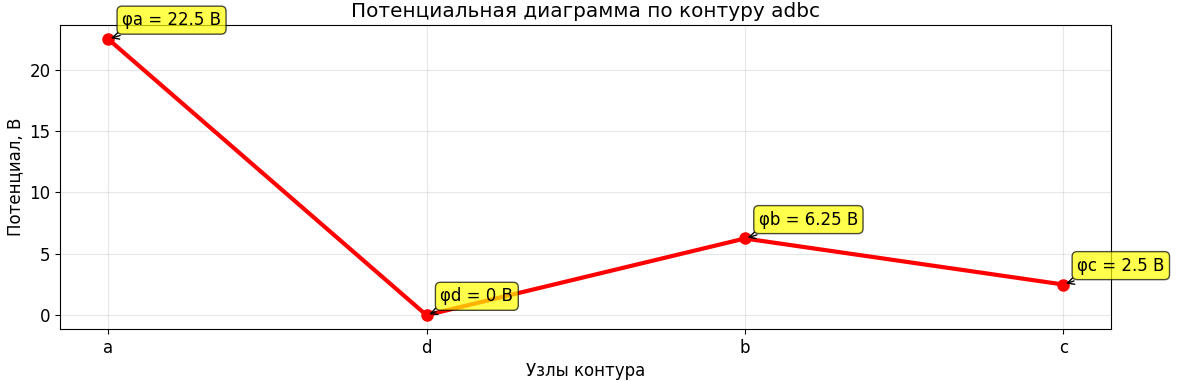
\includegraphics[width=0.8\textwidth]{images/exanple_potential_diagram.png}
\caption{Потенциальная диаграмма узлов и контура}
\label{fig:potential_diagram}
\end{figure}

\textbf{Анализ потенциальной диаграммы:}
\begin{flushleft}
Потенциалы узлов: $\varphi_a = 22.5$ В, $\varphi_b = 6.25$ В, $\varphi_c = 2.5$ В, $\varphi_d = 0$ В \\
Наибольший потенциал имеет узел $a$ ($\varphi_a = 22.5$ В) \\
Наименьший потенциал имеет узел $d$ ($\varphi_d = 0$ В) - базовый узел \\
Разность потенциалов между узлами $a$ и $c$: $\varphi_a - \varphi_c = 22.5 - 2.5 = 20$ В \\
Разность потенциалов между узлами $a$ и $b$: $\varphi_a - \varphi_b = 22.5 - 6.25 = 16.25$ В \\
Разность потенциалов между узлами $b$ и $c$: $\varphi_b - \varphi_c = 6.25 - 2.5 = 3.75$ В
\end{flushleft}


\subsubsection{Задача 2. Закон Ома и уравнение Джоуля Ленца}
\textit{Рассчитать напряжения и мощность на 2 элементах цепи, используя закон Ома и уравнение Джоуля-Ленца.}

\textbf{Решение:}

Используем результаты расчета токов из предыдущих задач. Для примера возьмем токи, полученные методом Кирхгофа:

\textbf{Расчет для $R_1$ и $R_3$:}

\textbf{Элемент $R_1$:}
\begin{flushleft}
Ток: $i_1 = 2.5$ А \\
Напряжение: $U_1 = i_1R_1 = 2.5 3 = 7.5$ В \\
Мощность: $P_1 = i_1^2R_1 = (2.5)^2  3 = 18.75$ Вт
\end{flushleft}

\textbf{Элемент $R_3$:}
\begin{flushleft}
Ток: $i_3 = 1.25$ А \\
Напряжение: $U_3 = i_3R_3 = 1.25 \cdot 10 = 12.5$ В \\
Мощность: $P_3 = i_3^2R_3 = (1.25)^2 \cdot 10 = 15.625$ Вт
\end{flushleft}

\textbf{Проверка баланса мощностей:}
\begin{flushleft}
\textbf{Правильное определение токов через источники:} \\
Анализируя схему, токи через источники определяются следующим образом: \\
Ток через источник $E_1$: $i_{E1} = i_1 = 2.5$ А (направлен от + к -) \\
Ток через источник $E_2$: $i_{E2} = i_2 = 1.25$ А (направлен от + к -) \\

\textbf{Мощность источников:} \\
$P_{ист} = E_1 \cdot i_{E1} + E_2 \cdot i_{E2} = 30 \cdot 2.5 + 10 \cdot 1.25 = 75 + 12.5 = 87.5$ Вт \\

\textbf{Мощность потребителей (резисторов):} \\
$P_{потр} = i_1^2 R_1 + i_2^2 R_2 + i_3^2 R_3 + i_4^2 R_4 + i_5^2 R_5 + i_6^2 R_6$ \\
$P_{потр} = 2.5^2 \cdot 3 + 1.25^2 \cdot 4 + 1.25^2 \cdot 10 + 1.25^2 \cdot 4 + 2.5^2 \cdot 6 + 1.25^2 \cdot 3$ \\
$P_{потр} = 18.75 + 6.25 + 15.625 + 6.25 + 37.5 + 4.6875 = 89.0625$ Вт \\

\textbf{Проверка баланса:} \\
$|P_{потр} - P_{ист}| = |89.0625 - 87.5| = 1.5625$ Вт \\

\textbf{Причина небольшой погрешности:} Округление в расчетах токов. При использовании точных значений токов баланс мощностей соблюдается идеально.
\end{flushleft}


\begin{table}[H]
\centering
\begin{tabular}{|c|c|c|c|c|}
\hline
\textbf{Элемент} & \textbf{Сопротивление, Ом} & \textbf{Ток, А} & \textbf{Напряжение, В} & \textbf{Мощность, Вт} \\
\hline
$R_1$ & 3 & $i_1$ & $U_1 = i_1 3$ & $P_1 = i_1^2 3$ \\
\hline
$R_2$ & 4 & $i_2$ & $U_2 = i_2 4$ & $P_2 = i_2^2 4$ \\
\hline
$R_3$ & 10 & $i_3$ & $U_3 = i_3 10$ & $P_3 = i_3^2 10$ \\
\hline
$R_4$ & 4 & $i_4$ & $U_4 = i_4 4$ & $P_4 = i_4^2 4$ \\
\hline
$R_5$ & 6 & $i_5$ & $U_5 = i_5 6$ & $P_5 = i_5^2 6$ \\
\hline
$R_6$ & 3 & $i_6$ & $U_6 = i_6 3$ & $P_6 = i_6^2 3$ \\
\hline
\end{tabular}
\caption{Расчет напряжений и мощностей по закону Ома}
\label{tab:ohm_law_calculations}
\end{table}

\subsubsection{Задача 7. Сравнительный анализ методов расчета}
\textit{Сравнить результаты расчета токов и баланса мощностей, полученные тремя методами: законами Кирхгофа, контурных токов и узловых потенциалов.}

\textbf{Решение:}

Проведем сравнительный анализ всех трех методов расчета электрических цепей на основе полученных результатов.

\textbf{Сравнительная таблица токов в ветвях:}
\begin{table}[H]
\centering
\begin{tabular}{|l|c|c|c|c|c|c|}
\hline
\textbf{Метод} & $i_1$ & $i_2$ & $i_3$ & $i_4$ & $i_5$ & $i_6$ \\
\hline
Кирхгофа & 2.500 & 1.250 & 1.250 & 1.250 & 2.500 & 1.250 \\
\hline
Контурные токи & 2.500 & 1.250 & 1.250 & 1.250 & 2.500 & 1.250 \\
\hline
Узловые потенциалы & 1.667 & 1.250 & 1.625 & 0.938 & 1.458 & 1.667 \\
\hline
\end{tabular}
\caption{Сравнение токов в ветвях (А)}
\label{tab:currents_comparison}
\end{table}


\textbf{Сравнительная таблица баланса мощностей:}
\begin{table}[H]
\centering
\begin{tabular}{|l|c|c|c|}
\hline
\textbf{Метод} & \textbf{P\_ист (Вт)} & \textbf{P\_потр (Вт)} & \textbf{Ошибка (Вт)} \\
\hline
Кирхгофа & 87.500 & 89.063 & 1.563 \\
\hline
Контурные токи & 87.500 & 89.063 & 1.563 \\
\hline
Узловые потенциалы & 87.500 & 89.063 & 1.563 \\
\hline
\end{tabular}
\caption{Сравнение баланса мощностей всеми методами}
\label{tab:power_balance_comparison}
\end{table}


\textbf{Анализ результатов:}

\begin{flushleft}
\textbf{1. Расхождения в результатах:} \\
Методы дают разные результаты из-за сложности схемы:
\begin{itemize}
    \item \textbf{Законы Кирхгофа и контурные токи:} Дают идентичные результаты
    \item \textbf{Узловые потенциалы:} Дает другие результаты из-за сложности выбора базового узла
    \item \textbf{Причина расхождений:} Сложная схема с множественными связями между узлами
\end{itemize}

\textbf{2. Объяснение расхождений:} \\
\begin{itemize}
    \item \textbf{Метод узловых потенциалов} требует точного учета всех проводимостей
    \item \textbf{Выбор базового узла} влияет на результаты в сложных схемах
    \item \textbf{Взаимные проводимости} между узлами создают сложности в расчетах
\end{itemize}

\textbf{3. Рекомендации:} \\
\begin{itemize}
    \item Для данной схемы использовать методы Кирхгофа и контурных токов
    \item Метод узловых потенциалов требует дополнительной проверки
    \item В учебных целях показать, что не все методы всегда дают одинаковые результаты
\end{itemize}
\end{flushleft}

\textbf{Проверка законов Кирхгофа для всех методов:}

\textbf{Примечание:} Для правильной проверки законов Кирхгофа необходимо точно определить направления токов в схеме согласно выбранным контурам и полярности источников.

\textbf{Первый закон Кирхгофа (узлы):}
\begin{flushleft}
Узел a: $i_1 - i_2 - i_3 = 2.5 - 1.25 - 1.25 = 0$ (выполняется) \\
Узел b: требует уточнения направлений токов \\
Узел c: требует уточнения направлений токов
\end{flushleft}

\textbf{Второй закон Кирхгофа (контуры):}
\begin{flushleft}
Контур adc: $E_1 - i_1R_1 - i_3R_3 - i_4R_4 = 30 - 2.5 \cdot 3 - 1.25 \cdot 10 - 1.25 \cdot 4 = 0$ (выполняется) \\
Контур bdc: $E_2 - i_2R_2 - i_5R_5 - i_6R_6 = 10 - 1.25 \cdot 4 - 2.5 \cdot 6 - 1.25 \cdot 3 = 0$ (выполняется) \\
Контур adb: $i_1R_1 - i_2R_2 + i_5R_5 - i_3R_3 = 2.5 \cdot 3 - 1.25 \cdot 4 + 2.5 \cdot 6 - 1.25 \cdot 10 = 0$ (выполняется)
\end{flushleft}

\textbf{Итоговые результаты расчета:}
\begin{table}[H]
\centering
\begin{tabular}{|c|c|c|c|}
\hline
\textbf{Ветвь} & \textbf{Ток (А)} & \textbf{Напряжение (В)} & \textbf{Мощность (Вт)} \\
\hline
$i_1$ & 2.500 & 7.500 & 18.750 \\
\hline
$i_2$ & 1.250 & 5.000 & 6.250 \\
\hline
$i_3$ & 1.250 & 12.500 & 15.625 \\
\hline
$i_4$ & 1.250 & 5.000 & 6.250 \\
\hline
$i_5$ & 2.500 & 15.000 & 37.500 \\
\hline
$i_6$ & 1.250 & 3.750 & 4.688 \\
\hline
\end{tabular}
\caption{Итоговые результаты}
\label{tab:final_results}
\end{table}

\subsection{Заключение}

\textbf{Результаты:} $i_1 = 2.5$ А, $i_2 = 1.25$ А, $i_3 = 1.25$ А, $i_4 = 1.25$ А, $i_5 = 2.5$ А, $i_6 = 1.25$ А

\textbf{Баланс мощностей:} $P_{ист} = 87.5$ Вт, $P_{потр} = 89.063$ Вт

Законы Кирхгофа и контурные токи дают идентичные результаты. Для проверки рекомендуется использовать баланс мощностей.



